\documentclass[letterpaper,11pt]{article}

% --- PAQUETES DE IDIOMA
\usepackage[spanish,mexico]{babel}
\addto\captionsspanish{\renewcommand{\contentsname}{Indice}}
\usepackage[utf8]{inputenc}
\usepackage{pmboxdraw}
\usepackage{csquotes}
\usepackage{iftex}

\usepackage{pdfpages}

% --- PAQUETES MATEMÁTICOS --
\usepackage{amsmath}
\usepackage{cancel}
\usepackage{mathrsfs}

% --- PAQUETES GRÁFICOS Y DE DISEÑO ---
\usepackage{graphicx}
\usepackage{float}
\usepackage{placeins}
\usepackage{needspace}
\usepackage{subcaption}
\usepackage[table]{xcolor}
\usepackage{makecell}
\usepackage{array}
\usepackage{tikz}
\usetikzlibrary{shapes.geometric, shapes.multipart, positioning, arrows.meta, calc, shadows, decorations.pathreplacing,babel}

% --- LISTAS ---
\usepackage{enumitem}

% --- PAQUETES DE CÓDIGO ---
\usepackage{listings}
% Configuración del estilo de listings
\definecolor{codebg}{rgb}{0.95,0.95,0.95}   
\definecolor{keyword}{rgb}{0.0,0.2,0.6}     
\definecolor{comment}{rgb}{0.25,0.5,0.35}   
\definecolor{string}{rgb}{0.6,0.0,0.0}      
\definecolor{number}{rgb}{0.5,0.0,0.5}      
\definecolor{codegray}{rgb}{0.5,0.5,0.5}
\definecolor{codepurple}{rgb}{0.58,0,0.82}
\definecolor{backcolour}{rgb}{0.95,0.95,0.95}
\definecolor{cmdblue}{RGB}{0, 114, 188}
\definecolor{cmdred}{RGB}{204, 0, 0}       
\definecolor{cmdgreen}{RGB}{13, 165, 13}   
\definecolor{cmdgray}{RGB}{128, 128, 128} 
\definecolor{bgcode}{RGB}{248, 248, 248} 
\definecolor{bgTerminal}{RGB}{30, 30, 30}
\definecolor{textTerminal}{RGB}{230, 230, 230}




\lstset{
  backgroundcolor=\color{backcolour},
  basicstyle=\ttfamily\small,
  keywordstyle=\color{blue}\bfseries,
  stringstyle=\color{codepurple},
  commentstyle=\color{codegray}\itshape,
  numbers=left,
  numberstyle=\tiny\color{codegray},
  frame=single,
  rulecolor=\color{black},
  breaklines=true,
  tabsize=4,
  showstringspaces=false,
  literate={á}{{\'a}}1
           {é}{{\'e}}1
           {í}{{\'i}}1
           {ó}{{\'o}}1
           {ú}{{\'u}}1
           {Á}{{\'A}}1
           {É}{{\'E}}1
           {Í}{{\'I}}1
           {Ó}{{\'O}}1
           {Ú}{{\'U}}1
           {ñ}{{\~n}}1
           {Ñ}{{\~N}}1
           {¿}{{\textquestiondown}}1
           {¡}{{\textexclamdown}}1
}

% Estilo para código en C
\lstdefinestyle{cstyle}{
  language=C,
  backgroundcolor=\color{backcolour},
  basicstyle=\ttfamily\small,
  keywordstyle=\color{blue}\bfseries,
    keywordstyle=[2]\color{yellow!70!orange}\bfseries,
    morekeywords=[2]{MPI_Init,MPI_Comm_size,MPI_Comm_rank,MPI_Send,MPI_Recv,MPI_Scatter,MPI_Gather,MPI_Bcast,MPI_Reduce,MPI_Finalize},
    emph={printf},
    emphstyle=\color{blue}\bfseries,
  stringstyle=\color{codepurple},
  commentstyle=\color{codegray}\itshape,
  numbers=left,
  numberstyle=\tiny\color{codegray},
  frame=single,
  rulecolor=\color{black},
  breaklines=true,
  tabsize=4,
  showstringspaces=false
}

\lstdefinestyle{salidaLinpeas}{
    basicstyle=\ttfamily\scriptsize\color{textTerminal},
    backgroundcolor=\color{bgTerminal},
    breaklines=true,
    breakatwhitespace=true,
    frame=single,
    rulecolor=\color{black!50},
    numbers=none,
    showstringspaces=false,
    tabsize=4,
    xleftmargin=0.5cm,
    xrightmargin=0.5cm,
    extendedchars=false,
    literate={═}{{\textSFxliii}}1
             {║}{{\textSFxxiv}}1
             {╔}{{\textSFxxxix}}1
             {╗}{{\textSFxxv}}1
             {╚}{{\textSFxxxviii}}1
             {╝}{{\textSFxxvi}}1
             {╣}{{\textSFxxiii}}1
}  
\lstdefinestyle{consolaSeguridad}{
    language=bash,
    basicstyle=\ttfamily\footnotesize,
    backgroundcolor=\color{bgcode},
    % Herramientas y comandos de la práctica
    morekeywords={subfinder, make, scp, httpx, hydra, ssh, id, nuclei, dig, whois, grep, awk, sort, cut, sed, tr, nano, wc, head, echo, sudo, nmap, wget, curl, ip,
                  whoami, file, cat, cp, chown, chmod, sha256sum, apt-get, john, unshadow, su, pwnkit},
    alsoletter={-},
    keywordstyle=\color{cmdblue}\bfseries,
    % Palabras reservadas de ciclos Bash
    emph={for, in, do, done, while, read},
    emphstyle=\color{cmdred}\bfseries,
    stringstyle=\color{cmdgreen},
    commentstyle=\color{cmdgray}\itshape,
    showstringspaces=false,
    breaklines=true,
    breakatwhitespace=false,
    frame=single,
    rulecolor=\color{black!30},
    numbers=none,
    literate={-}{{\textcolor{black}{-}}}1 % Evita que los guiones de parámetros se coloreen
}

% Definición del lenguaje Python para listings
\lstdefinelanguage[LAB]{Python}{
    morekeywords={False, None, True, and, as, assert, async, await, break,
                                class, continue, def, del, elif, else, except, finally,
                                for, from, global, if, import, in, is, lambda, nonlocal,
                                not, or, pass, raise, return, try, while, with, yield,
                                machine, Pin, PWM, ADC, Timer, sleep_ms, sleep_us},
    morecomment=[l]{\#},
    morestring=[b]",
    morestring=[b]',
    sensitive=true
}

% Definición del lenguaje Makefile para listings
\lstdefinelanguage{Makefile}{
    morekeywords={all, setup, clean, conversion-mod.so, pwnkit},
    morecomment=[l]{\#},
    morestring=[b]',
    morestring=[b]",
    sensitive=true
}

% Estilo para salidas de consola/terminal
\lstdefinestyle{output}{
  backgroundcolor=\color{black!5},
  basicstyle=\ttfamily\footnotesize,
  numbers=none,
  frame=single,
  rulecolor=\color{black!30},
  breaklines=true,
  tabsize=4,
  showstringspaces=false,
  xleftmargin=0.5cm,
  xrightmargin=0.5cm
}

% --- ESTILOS PARA DIAGRAMAS DE FLUJO (TIKZ) ---
\tikzset{
  startstop/.style={rectangle, rounded corners, minimum width=3cm, minimum height=1cm,text centered, draw=black, fill=red!30},
  process/.style={rectangle, minimum width=3cm, minimum height=1cm, text centered, draw=black, fill=orange!30},
  decision/.style={diamond, aspect=2, minimum width=3cm, minimum height=1cm, text centered, draw=black, fill=green!30},
  io/.style={trapezium, trapezium left angle=70, trapezium right angle=110, minimum width=3cm, minimum height=1cm, text centered, draw=black, fill=blue!30},
  arrow/.style={thick,->,>=stealth}
}


\definecolor{azulresultado}{HTML}{0072C6}
\definecolor{rojoacarreo}{HTML}{FF0000}

% --- RUTAS DE IMÁGENES ---
\graphicspath{{img/}{portada_img/}}

\definecolor{armblue}{RGB}{0, 113, 188}

% --- ÍNDICE CON PUNTOS ---
\usepackage{tocloft}
\renewcommand{\cftsecleader}{\cftdotfill{\cftdotsep}}

% --- CONFIGURACIÓN DE PÁGINA (GEOMETRÍA) ---
\usepackage[
    left=25mm, 
    right=25mm,
    top=35mm,
    bottom=30mm,
    headheight=77pt, 
    papersize={21.59cm,27.94cm}
]{geometry}

% --- FORMATO DE TEXTO ---
\usepackage{setspace}
\onehalfspacing
\usepackage{parskip} 
\usepackage{lipsum}  

% --- VARIABLES GLOBALES ---
\newcommand{\materia}{}

% --- ENCABEZADOS Y PIES DE PÁGINA ---
\usepackage{fancyhdr}
\pagestyle{fancy}
\fancyhf{} 
\fancyhead[L]{
\includegraphics[height=1.5cm]{portada_img/der.png}}
\fancyhead[R]{
\includegraphics[height=1.5cm]{portada_img/izq.png}}
\fancyfoot[C]{\thepage} 

\renewcommand{\headrulewidth}{0.4pt} 
\renewcommand{\footrulewidth}{0pt}  

% --- BIBLIOGRAFÍA ---
\usepackage[backend=biber, style=apa, sortcites, url=true]{biblatex}
\addbibresource{referencias.bib}

% --- HIPERVÍNCULOS ---
\usepackage{hyperref}
\hypersetup{
    colorlinks=true,
    linkcolor=blue,
    citecolor=blue,
    filecolor=magenta,
    urlcolor=cyan
}


\fancypagestyle{estiloindice}{
  \fancyhf{} 
  \fancyhead[L]{
\includegraphics[height=1.5cm]{portada_img/der.png}}
  \fancyhead[R]{
\includegraphics[height=1.5cm]{portada_img/izq.png}}
  \renewcommand{\headrulewidth}{0.4pt} 
  \renewcommand{\footrulewidth}{0pt}
}


% --- CADENAS DE HASHES: CONSERVAR CARACTERES Y PERMITIR SALTOS ---
\lstdefinestyle{hashCredencial}{
  style=output,
  basicstyle=\ttfamily\footnotesize,
  columns=fullflexible,
  keepspaces=true,
  breaklines=true,
  breakatwhitespace=false,
  xleftmargin=0pt,
  xrightmargin=0pt,
  postbreak=\mbox{\textcolor{codegray}{$\hookrightarrow$}\space}
}

\begin{document}
\setlength{\emergencystretch}{1em}
\hypersetup{pageanchor=false}
\thispagestyle{empty} % Sin encabezado ni pie en la portada

% --- ENCABEZADO DE PORTADA (TABLA DE 3 COLUMNAS) ---
\begin{center}
    % La tabla usa 'm' para centrar verticalmente las imagenes y el texto
    \begin{tabular}{m{0.15\textwidth} m{0.60\textwidth} m{0.15\textwidth}}
        % Logo Izquierdo (UNAM)
        
\includegraphics[width=2cm]{portada_img/der.png} & 
        
        % Titulo Central
        \centering\Huge\textbf{Universidad Nacional Autonoma de Mexico} &
        
        % Logo Derecho (Facultad)
        \raggedleft
\includegraphics[width=2cm]{portada_img/izq.png}
    \end{tabular}
\end{center}

\vspace{0.3cm}

% --- INFORMACION DEL REPORTE ---
\begin{center}
    {\LARGE \textbf{Facultad de Ingenieria}}\\[1cm]

    {\LARGE \textbf{Alumno:}}\\[0.3cm]
    {\Large Lara Hernandez Angel Husiel - 320060829} \\[1cm]


    {\LARGE \textbf{Seguridad informatica basica}} \\[1cm]

	{\LARGE Semestre: 2027-1} \\[1cm]
    
    {\LARGE \textbf{Practica 5}}\\[0.5cm]

    {\LARGE {Credential Access}}\\[1cm]


    {\Large \textbf{Fecha de Entrega:}}\\[0.2cm]
    {\Large 31 de Octubre del 2026 }
\end{center}
\newpage
{\hypersetup{linkcolor=black}\tableofcontents}
\thispagestyle{estiloindice}
\newpage
\thispagestyle{fancy}
\setcounter{page}{1}
\hypersetup{pageanchor=true}
\singlespacing
\section{Desarrollo}

\subsection{Identificacion de las direcciones IP y revision de conectividad}

Ahora bien, antes de conectarnos al servidor, lo primero que
hacemos es revisar la direccion IP de nuestra maquina. Para
esto, el comando que ponemos en la terminal de EvilBox es el
siguiente:

\begin{lstlisting}[style=consolaSeguridad]
ip a
\end{lstlisting}

Lo que hace este comando es mostrar las interfaces de red y sus
direcciones. Donde en este caso, la interfaz \texttt{ens33}
tiene la direccion \texttt{192.168.177.128/24}. Esto nos dice
que el segmento que tenemos que revisar es
\texttt{192.168.177.0/24}; el prefijo \texttt{/24} corresponde a
la mascara \texttt{255.255.255.0}.

Despues de esto, ejecutamos el comando de nmap que se pide en la
guia, pero cambiando el segmento por el que realmente estamos
utilizando:

\begin{lstlisting}[style=consolaSeguridad]
sudo nmap -sP 192.168.177.0/24
\end{lstlisting}

Donde \texttt{sudo} permite ejecutar el escaneo con permisos de
administracion y la bandera \texttt{-sP} realiza el
descubrimiento de equipos activos. Esta opcion tambien se conoce
como \texttt{-sn}, y en este caso se utiliza para encontrar los
equipos que responden, sin realizar un escaneo de todos sus
puertos.

\begin{figure}[H]
    \centering
    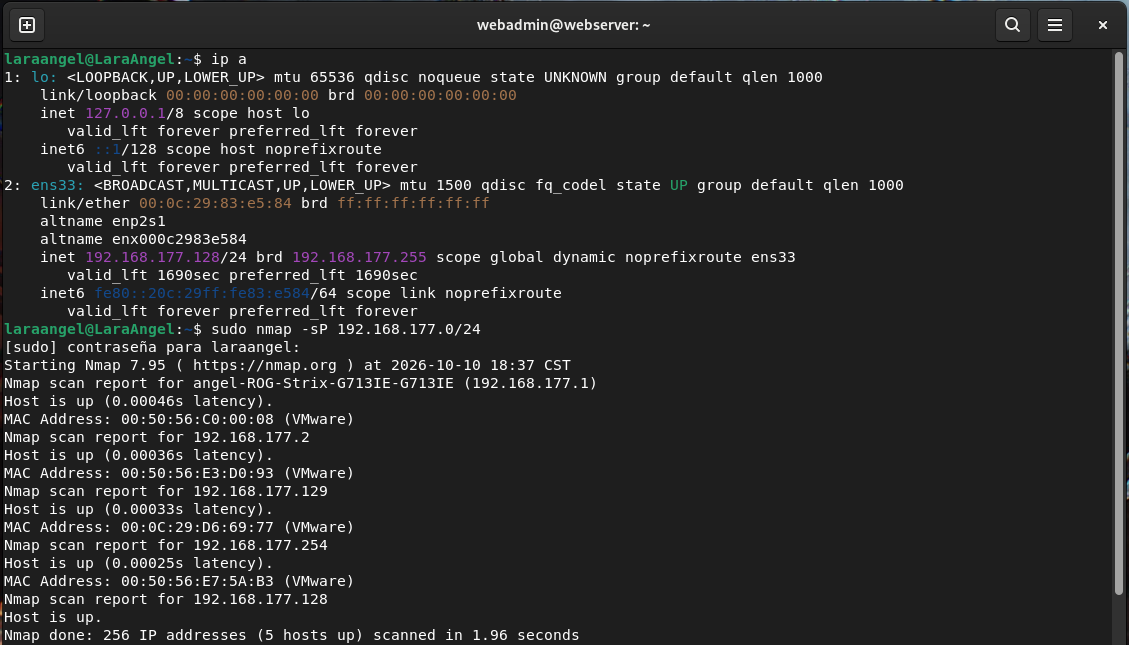
\includegraphics[width=\textwidth]{img/image1.png}
    \caption{Direccion IP de EvilBox y descubrimiento de los equipos del segmento de red.}
    \label{fig:red}
\end{figure}

La salida nos arroja cinco equipos activos. Donde en este caso,
el servidor que nos interesa tiene la IP
\texttt{192.168.177.129}, que es la misma que se habia utilizado
en las practicas anteriores. No obstante, para confirmar que
corresponde a webserver, el siguiente paso es establecer la
sesion SSH y revisar el equipo al que entramos.

\subsection{Conexion por SSH con las credenciales de la practica 3}

Para poder conectarnos a webserver, utilizamos las credenciales
que se obtuvieron con Hydra en la practica 3. Recordando que el
usuario es \texttt{webadmin}, la contraseña es \texttt{toronto}
y el servicio SSH se encuentra en el puerto \texttt{13337}, el
comando que se pone es el siguiente:

\begin{lstlisting}[style=consolaSeguridad]
ssh webadmin@192.168.177.129 -p 13337
\end{lstlisting}

Lo que hace este comando es abrir una sesion remota con el
usuario \texttt{webadmin} en la direccion del servidor. La
bandera \texttt{-p} indica el puerto de SSH, esto porque aqui no
se esta utilizando el puerto 22. Despues, cuando la terminal
solicita la contraseña, se escribe \texttt{toronto}.

\begin{figure}[H]
    \centering
    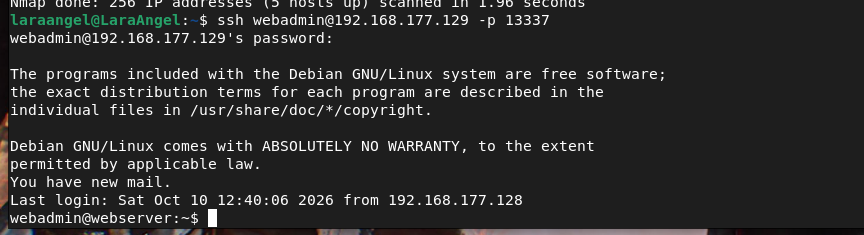
\includegraphics[width=\textwidth]{img/image2.png}
    \caption{Conexion por SSH al servidor con el usuario webadmin.}
    \label{fig:ssh}
\end{figure}

\subsection{Escalacion de privilegios y comprobacion del usuario root}

Ahora bien, estar conectados como \texttt{webadmin} no significa
que ya tengamos permisos de administracion. Para poder revisar
el archivo shadow, primero es necesario recuperar la terminal
como \texttt{root}, utilizando la vulnerabilidad que ya se habia
identificado en la practica 4, siendo esta
\textbf{CVE-2021-4034}, conocida como \textbf{PwnKit}.

Como los archivos del exploit ya se habian transferido a
webserver en la practica anterior, se vuelve a utilizar el mismo
comando de la practica anterior:

\begin{lstlisting}[style=consolaSeguridad]
make all && ./pwnkit && make clean
\end{lstlisting}

Para esto, \texttt{make all} prepara y compila los archivos que
necesita el exploit, despues \texttt{./pwnkit} ejecuta el
programa y \texttt{make clean} realiza la limpieza cuando
termina la ejecucion anterior. Los simbolos \texttt{\&\&} hacen
que cada parte se ejecute solamente si la anterior termino
correctamente. De hecho, mientras estamos dentro de la terminal
que abrio el exploit, el proceso todavia no ha regresado a la
sesion original, por lo que la limpieza final queda para cuando
se salga de esa terminal.

Despues de ejecutarlo, comprobamos el usuario con el siguiente
comando:

\begin{lstlisting}[style=consolaSeguridad]
whoami
\end{lstlisting}

\begin{lstlisting}[style=output]
root
\end{lstlisting}

\begin{figure}[H]
    \centering
    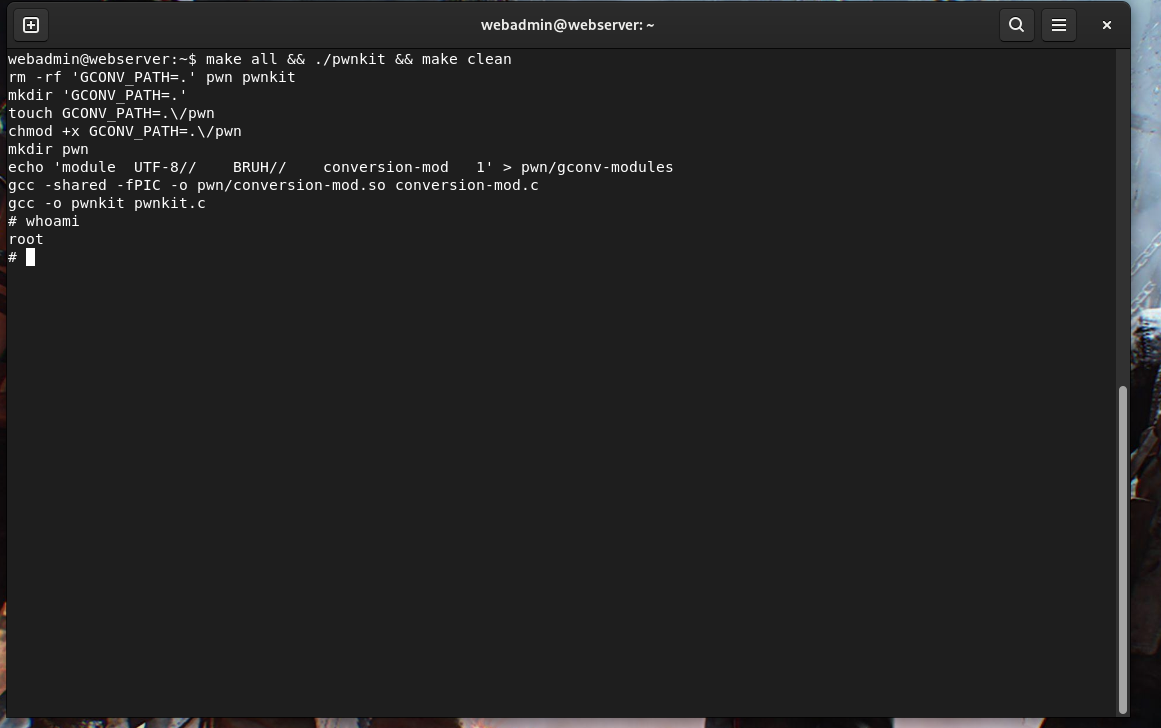
\includegraphics[width=\textwidth,trim=0bp 410bp 0bp 0bp,clip]{img/image3.png}
    \caption{Ejecucion del exploit y comprobacion del usuario root con whoami.}
    \label{fig:root}
\end{figure}

Donde en este caso, el comando whoami nos arroja root, por lo
que con esto se comprueba que se logro hacer la escalacion de
privilegios y ya tenemos los permisos necesarios para revisar
los archivos del servidor.

\subsection{Identificacion y lectura de los archivos passwd y shadow}

Una vez que tenemos la terminal como root, lo siguiente es
identificar los dos archivos que pide la guia. Para esto,
primero utilizamos el comando \texttt{file}, el cual nos dice
que tipo de contenido tiene cada archivo:

\begin{lstlisting}[style=consolaSeguridad]
file /etc/passwd
file /etc/shadow
\end{lstlisting}

\begin{lstlisting}[style=output]
/etc/passwd: ASCII text
/etc/shadow: ASCII text
\end{lstlisting}

\begin{figure}[H]
    \centering
    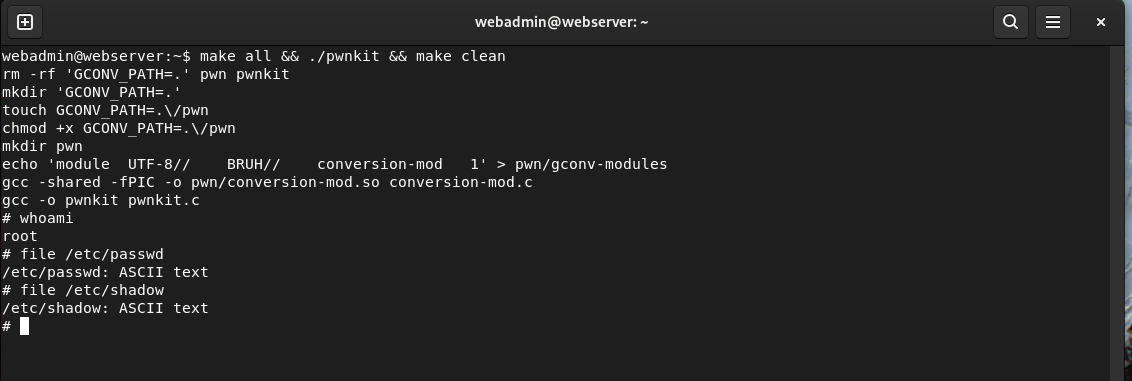
\includegraphics[width=\textwidth,trim=0bp 40bp 0bp 235bp,clip]{img/image4.png}
    \caption{Identificacion de passwd y shadow como archivos de texto.}
    \label{fig:file}
\end{figure}

Esto nos dice que ambos archivos contienen texto, por lo que
podemos revisar su contenido desde la terminal. No obstante,
esto no quiere decir que las contraseñas esten guardadas en
claro. Para ver que contiene el primero, ponemos el siguiente
comando:

\begin{lstlisting}[style=consolaSeguridad]
cat /etc/passwd
\end{lstlisting}

\begin{figure}[H]
    \centering
    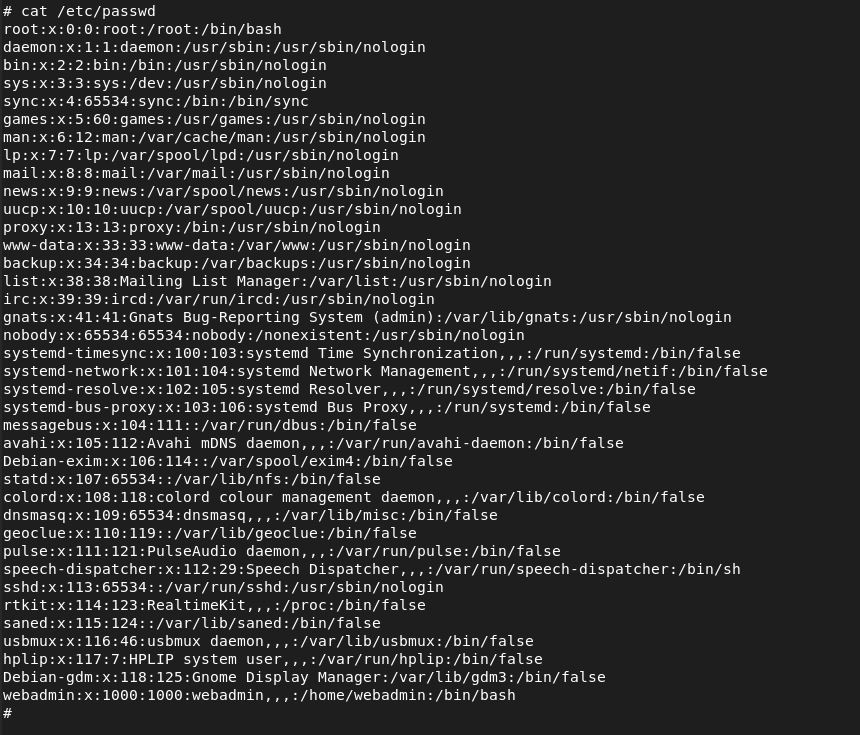
\includegraphics[width=0.88\textwidth]{img/image5.png}
    \caption{Listado de cuentas del sistema en el archivo /etc/passwd.}
    \label{fig:passwd}
\end{figure}

Lo que hace \texttt{cat} es imprimir el contenido del archivo.
Donde en este caso podemos ver tanto cuentas de servicios, como
\texttt{www-data} y \texttt{sshd}, como las cuentas
\texttt{root} y \texttt{webadmin}. Las lineas de estos dos
usuarios son las siguientes:

\begin{lstlisting}[style=output]
root:x:0:0:root:/root:/bin/bash
webadmin:x:1000:1000:webadmin,,,:/home/webadmin:/bin/bash
\end{lstlisting}

Para entender estas lineas, los campos estan separados por dos
puntos y representan lo siguiente:

\begin{enumerate}
    \item \textbf{Nombre de usuario:} identifica la cuenta,
    siendo root o webadmin en estos ejemplos.
    \item \textbf{Campo de contraseña:} la \texttt{x} indica que
    la informacion de la contraseña se encuentra en shadow.
    \item \textbf{UID:} es el identificador del usuario. Para
    root es 0 y para webadmin es 1000.
    \item \textbf{GID:} es el identificador del grupo principal,
    siendo 0 y 1000 respectivamente.
    \item \textbf{Comentario:} contiene informacion descriptiva
    de la cuenta.
    \item \textbf{Directorio personal:} es \texttt{/root} o
    \texttt{/home/webadmin}.
    \item \textbf{Shell:} indica el interprete de comandos, que
    en los dos casos es \texttt{/bin/bash}.
\end{enumerate}

Ahora bien, para ver los hashes de las contraseñas, revisamos el
otro archivo:

\begin{lstlisting}[style=consolaSeguridad]
cat /etc/shadow
\end{lstlisting}

\begin{figure}[H]
    \centering
    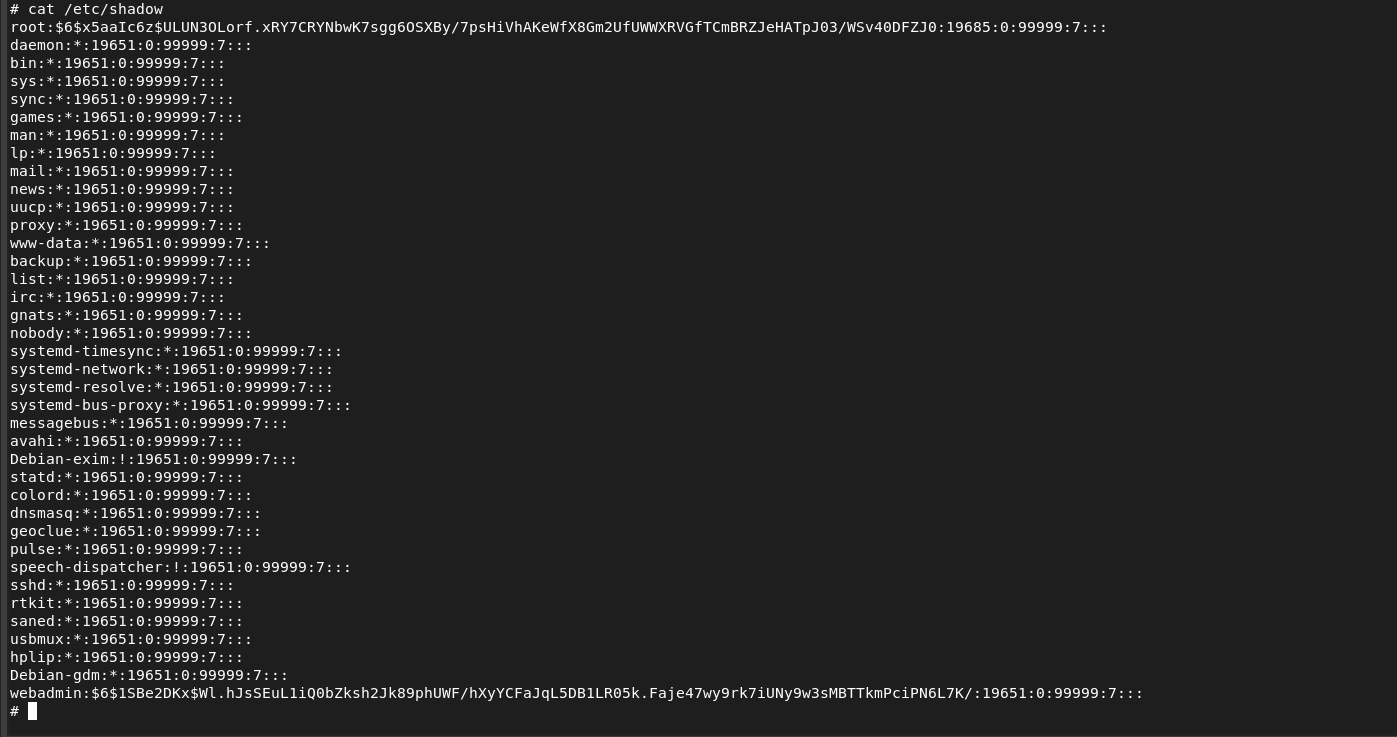
\includegraphics[width=\textwidth]{img/image6.png}
    \caption{Contenido de /etc/shadow y hashes de las cuentas root y webadmin.}
    \label{fig:shadow}
\end{figure}

Este archivo contiene el nombre de la cuenta, el campo de
contraseña y los datos de vigencia. Despues del hash aparecen la
fecha del ultimo cambio, la edad minima y maxima de la
contraseña, los dias de advertencia, el periodo de inactividad,
la expiracion de la cuenta y un campo reservado. La fecha del
ultimo cambio se expresa en dias desde el 1 de enero de 1970.

De igual forma, se pueden ver cuentas cuyo segundo campo es
\texttt{*} o \texttt{!}. Estos valores no son contraseñas en
claro ni hashes que se puedan probar como los de root y
webadmin; indican que la autenticacion mediante contraseña Unix
no esta disponible para esas entradas. Esto no implica que todos
los servicios asociados esten detenidos.

Para los dos usuarios que nos interesan, el campo comienza con
\texttt{\$6\$}. Esto corresponde al formato
\textbf{SHA512-crypt}. La cadena incluye el identificador del
metodo, una sal y el resultado del calculo. La sal hace que el
resultado dependa de un valor adicional propio de la contraseña
almacenada, por lo que no basta con aplicar un SHA512 simple al
texto de la contraseña.

Donde en este caso, la sal de root es \texttt{x5aaIc6z} y la de
webadmin es \texttt{1SBe2DKx}. Los hashes completos se muestran
en las actividades 3 y 4, esto para conservar todos sus
caracteres y poder distinguirlos de los hashes SHA256 de los
archivos.

\subsection{Copia de passwd y shadow al equipo EvilBox}

Ahora bien, para poder utilizar John, primero es necesario
copiar los archivos a nuestra maquina EvilBox, esto por que las
pruebas se van a realizar en esta maquina. Para esto, se
utilizan las copias llamadas \texttt{passwd.txt} y
\texttt{shadow.txt}, que se encuentran en el directorio
\texttt{/home/webadmin} del servidor.

Para preparar las copias, se puede utilizar el siguiente
procedimiento desde root, esto para copiar los archivos al
directorio de webadmin y darle acceso a las copias:

\begin{lstlisting}[style=consolaSeguridad]
cp /etc/passwd /home/webadmin/passwd.txt
cp /etc/shadow /home/webadmin/shadow.txt
chown webadmin:webadmin /home/webadmin/passwd.txt /home/webadmin/shadow.txt
chmod 600 /home/webadmin/passwd.txt /home/webadmin/shadow.txt
\end{lstlisting}

Lo que hace \texttt{cp} es crear las copias. Despues,
\texttt{chown} permite que webadmin sea el propietario de esos
archivos y \texttt{chmod 600} deja permisos de lectura y
escritura solamente para ese propietario. Esto se aplica a las
copias, para que puedan transferirse con la cuenta que ya
tenemos, manteniendo los archivos originales en \texttt{/etc}.

Despues de esto, desde nuestra maquina EvilBox, se copian los
archivos por medio de ssh, donde los comandos son los
siguientes:

\begin{lstlisting}[style=consolaSeguridad]
scp -P 13337 webadmin@192.168.177.129:/home/webadmin/passwd.txt .
scp -P 13337 webadmin@192.168.177.129:/home/webadmin/shadow.txt .
\end{lstlisting}

Donde \texttt{scp} permite transferir archivos por SSH,
\texttt{-P} indica el puerto del servicio y el punto final
significa que se guardan en el directorio actual de EvilBox. Hay
que tener en cuenta que aqui la bandera del puerto es
\texttt{-P} mayuscula, mientras que en el comando \texttt{ssh}
se utilizo \texttt{-p} minuscula.

\begin{figure}[H]
    \centering
    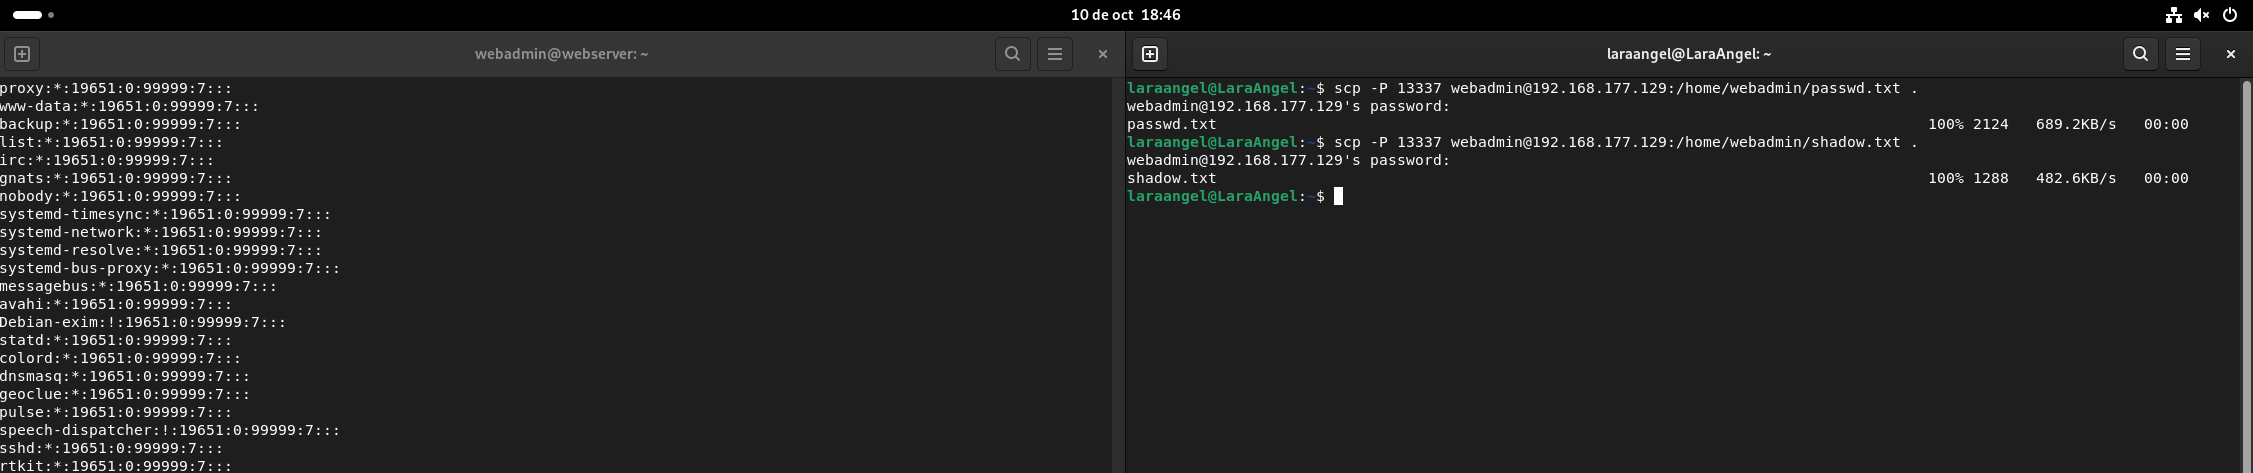
\includegraphics[width=\textwidth,trim=1120bp 250bp 0bp 0bp,clip]{img/image7.png}
    \caption{Transferencia de passwd.txt y shadow.txt desde webserver hacia EvilBox.}
    \label{fig:scp}
\end{figure}

La consola muestra que ambos archivos llegaron al 100\%, donde
\texttt{passwd.txt} tiene 2124 bytes y \texttt{shadow.txt} tiene
1288 bytes. No obstante, para verificar que el contenido
corresponde completamente a los originales, lo siguiente es
comparar sus hashes.

\subsection{Verificacion de integridad con SHA256}

Ahora bien, para revisar que los archivos se copiaron
correctamente, utilizamos \texttt{sha256sum}. Este comando
calcula un resumen SHA256 del contenido de cada archivo. Si el
original y la copia tienen el mismo resumen, la comparacion nos
permite verificar la integridad de lo que se transfirio.

Primero, en la terminal root de webserver, los comandos son los
siguientes:

\begin{lstlisting}[style=consolaSeguridad]
sha256sum /etc/passwd
sha256sum /etc/shadow
\end{lstlisting}

Por otro lado, en la terminal de EvilBox, se revisan los
archivos que se descargaron:

\begin{lstlisting}[style=consolaSeguridad]
sha256sum passwd.txt shadow.txt
\end{lstlisting}

\begin{figure}[H]
    \centering
    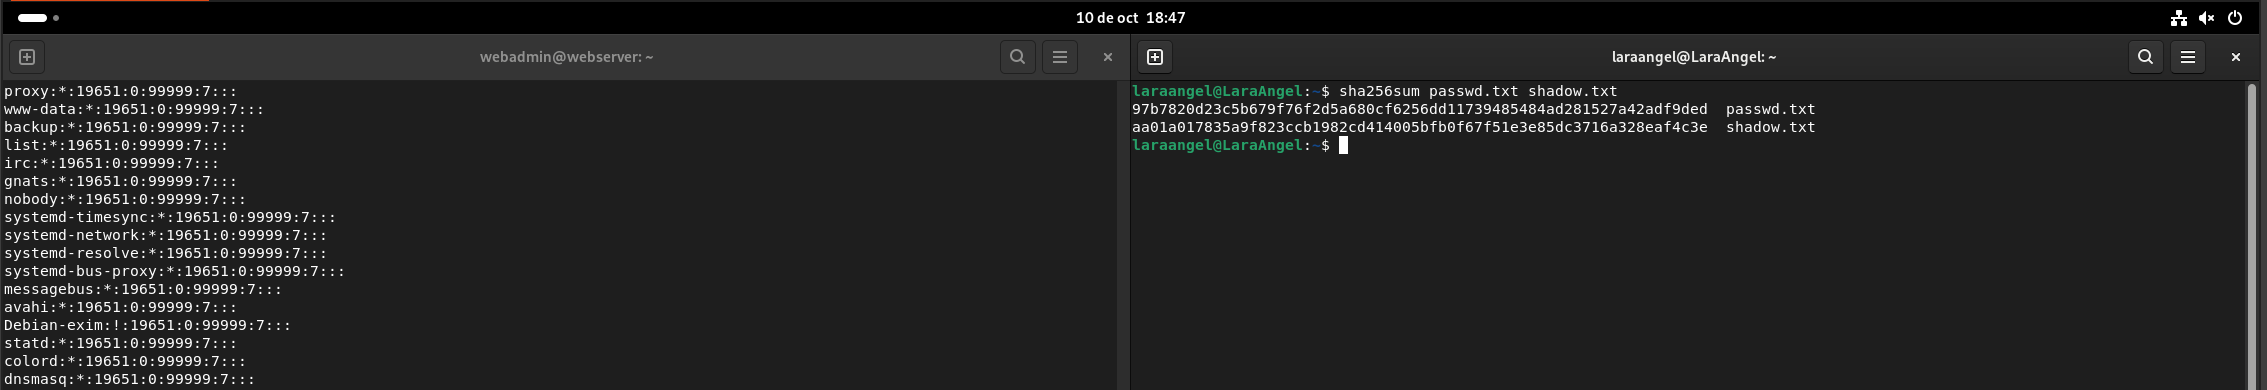
\includegraphics[width=\textwidth,trim=1130bp 205bp 0bp 0bp,clip]{img/image8.png}
    \caption{Calculo de los hashes SHA256 de los archivos recibidos en EvilBox.}
    \label{fig:sha_copias}
\end{figure}

\begin{figure}[H]
    \centering
    \begin{subfigure}{\textwidth}
        \centering
        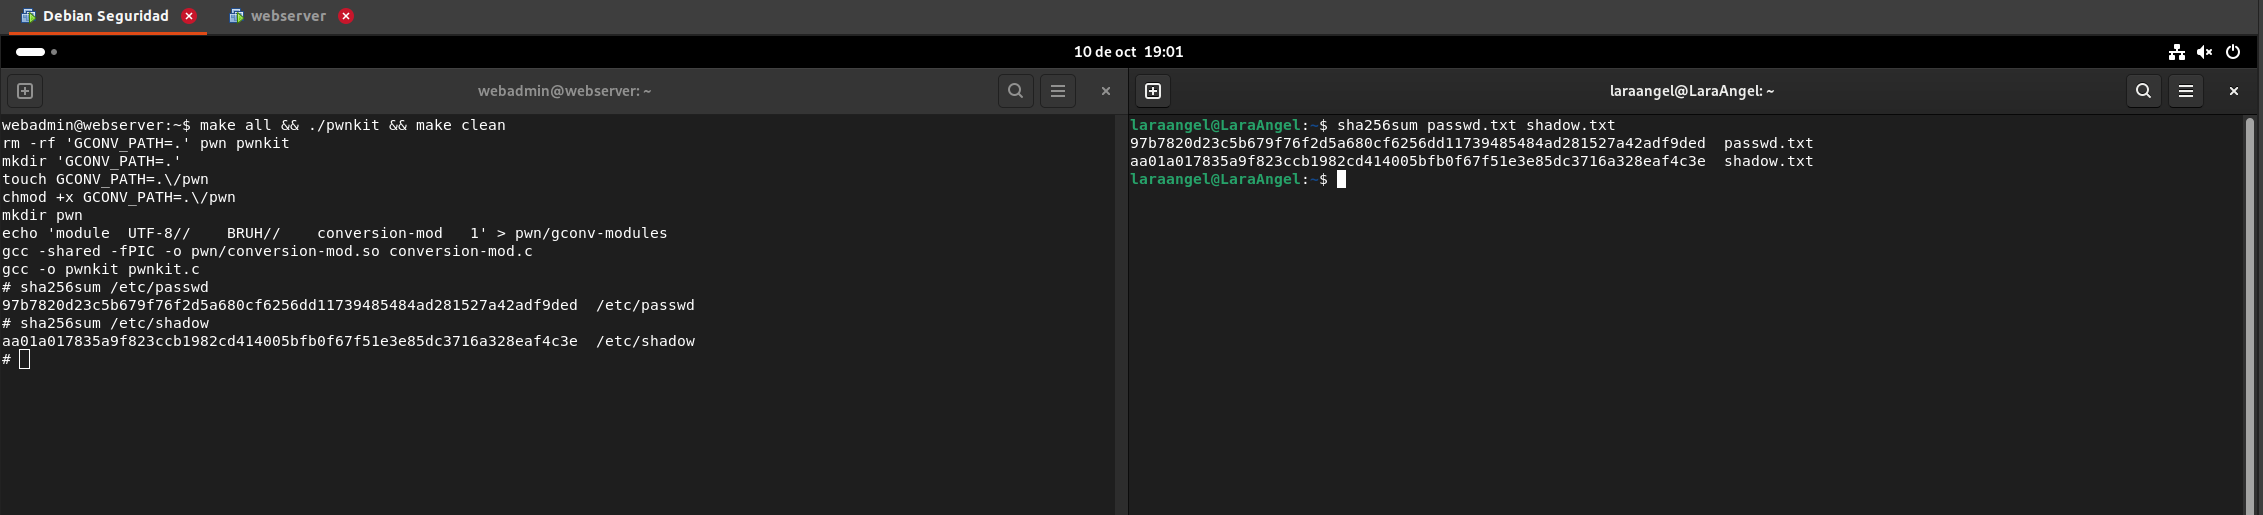
\includegraphics[width=\textwidth,trim=0bp 125bp 1140bp 270bp,clip]{img/image13.png}
        \caption{Hashes de los archivos originales en la terminal root de webserver.}
    \end{subfigure}
    \par\medskip
    \begin{subfigure}{\textwidth}
        \centering
        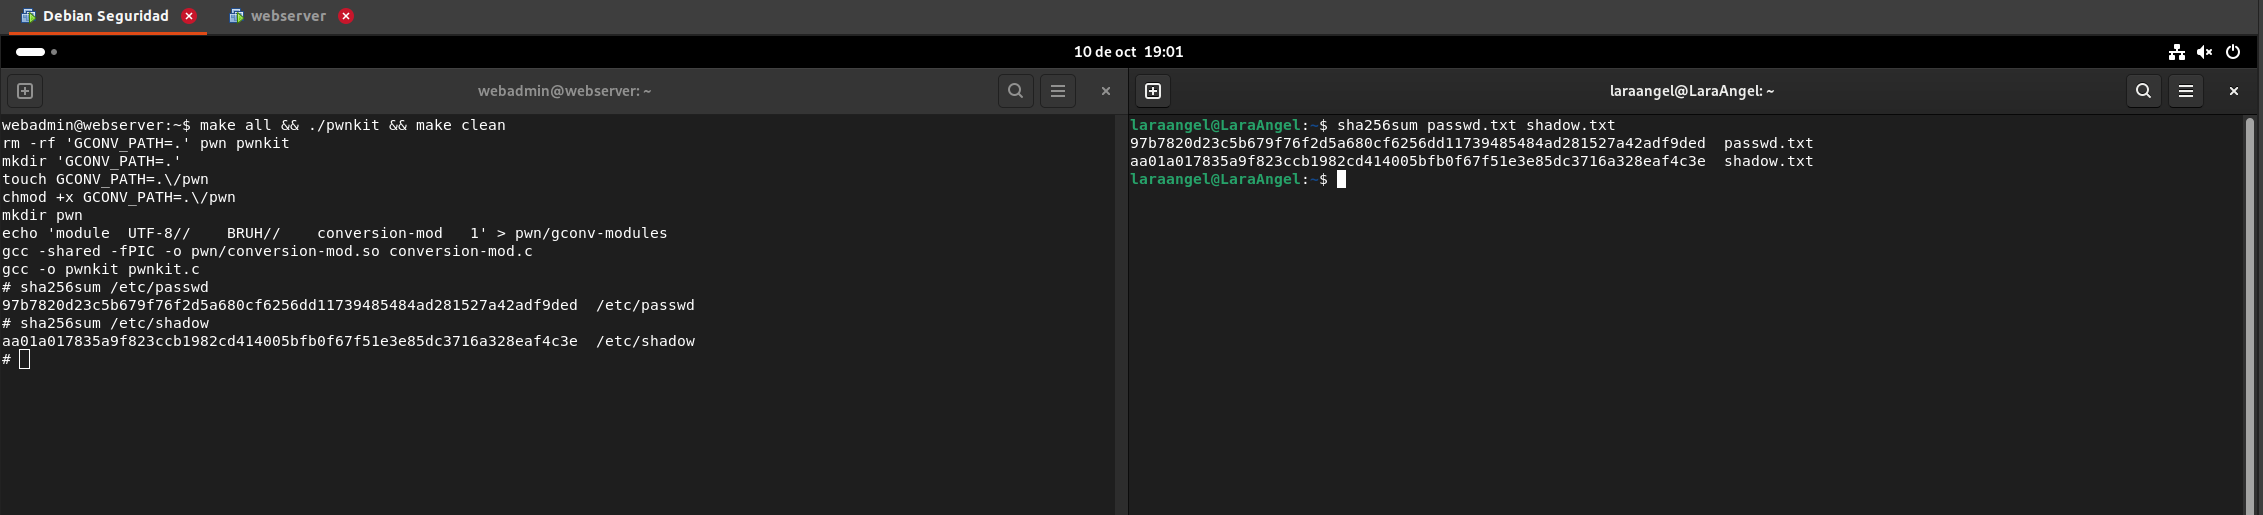
\includegraphics[width=\textwidth,trim=1125bp 315bp 0bp 95bp,clip]{img/image13.png}
        \caption{Hashes de las copias en la terminal local de EvilBox.}
    \end{subfigure}
    \caption{Comparacion entre los archivos originales y las copias transferidas.}
    \label{fig:integridad}
\end{figure}

Donde en este caso, los valores que aparecen en ambos equipos
son los siguientes:

\Needspace{4\baselineskip}
\textbf{SHA256 de passwd y passwd.txt:}
\begin{lstlisting}[style=hashCredencial]
97b7820d23c5b679f76f2d5a680cf6256dd11739485484ad281527a42adf9ded
\end{lstlisting}

\Needspace{4\baselineskip}
\textbf{SHA256 de shadow y shadow.txt:}
\begin{lstlisting}[style=hashCredencial]
aa01a017835a9f823ccb1982cd414005bfb0f67f51e3e85dc3716a328eaf4c3e
\end{lstlisting}

Con esto podemos ver que la copia de cada archivo coincide con
su original. Ademas de que, es importante distinguir que estamos
calculando aqui: el SHA256 corresponde al archivo completo,
mientras que el hash guardado dentro de shadow corresponde a la
contraseña de un usuario. Son resultados de operaciones
diferentes.

\subsection{Instalacion y comprobacion de John the Ripper}

Despues de tener los archivos en EvilBox, lo siguiente es
revisar que John the Ripper este instalado. Para esto se utiliza
el comando que viene en la guia:

\begin{lstlisting}[style=consolaSeguridad]
sudo apt-get install john
\end{lstlisting}

Lo que hace \texttt{apt-get install} es solicitar la instalacion
del paquete \texttt{john}. Donde en este caso, la consola nos
dice que John ya esta instalado y que la version del paquete es
\texttt{1.9.0-2}, por lo que no fue necesario instalar un
paquete nuevo.

\begin{figure}[H]
    \centering
    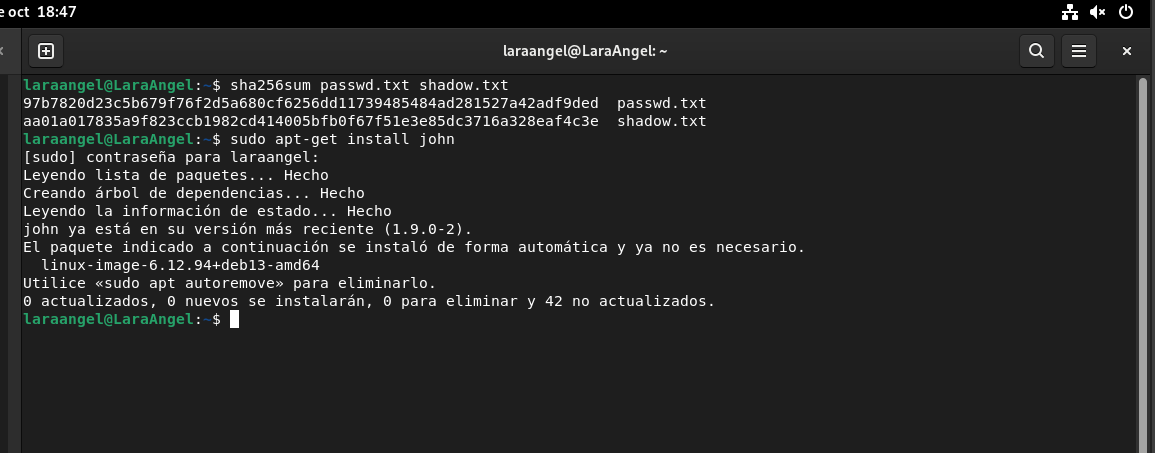
\includegraphics[width=\textwidth]{img/image9.png}
    \caption{Comprobacion del paquete John the Ripper en EvilBox.}
    \label{fig:john_instalado}
\end{figure}

Ahora bien, esta herramienta permite probar candidatos de
contraseña contra los hashes obtenidos. A diferencia de lo
realizado con Hydra en la practica 3, aqui las pruebas se hacen
con los archivos locales, por lo que no se necesita abrir una
conexion SSH por cada contraseña que se intenta. A este
procedimiento se le llama \textit{off-line cracking}.

\subsection{Fusion de los archivos con unshadow}

Para que John tenga tanto la informacion de las cuentas como sus
hashes, primero se fusionan los contenidos de passwd y shadow.
En nuestra ejecucion, el comando que se utiliza es el siguiente:

\begin{lstlisting}[style=consolaSeguridad]
/usr/sbin/unshadow passwd.txt shadow.txt > unshadow.txt
\end{lstlisting}

Donde \texttt{/usr/sbin/unshadow} es la ruta del programa que se
utiliza para combinar los archivos. Primero se le pasa
\texttt{passwd.txt}, despues \texttt{shadow.txt}, y el simbolo
\texttt{>} guarda la salida en \texttt{unshadow.txt}. La
combinacion relaciona los datos de cada cuenta con su campo de
contraseña.

Con esto, la informacion de los dos archivos se queda en
\texttt{unshadow.txt}, que es el archivo que se le va a pasar a
John para que pueda probar las contraseñas.

\subsection{Prueba de contraseñas con el diccionario local}

Ahora bien, teniendo el archivo \texttt{unshadow.txt}, es
necesario pasarle a John el diccionario de contraseñas. Donde en
este caso se utiliza el archivo
\texttt{contrasenas\_limpias.txt}, por lo que el comando es el
siguiente:

\begin{lstlisting}[style=consolaSeguridad]
/usr/sbin/john --wordlist=contrasenas_limpias.txt unshadow.txt
\end{lstlisting}

Lo que hace la opcion \texttt{--wordlist} es indicarle el
archivo con los candidatos que se van a probar. Para esto, John
calcula el resultado de cada candidato con el metodo y la sal
correspondientes, y busca una coincidencia con los hashes
cargados. Por lo tanto, se esta encontrando una contraseña que
coincide; no se esta invirtiendo directamente el hash.

\begin{figure}[H]
    \centering
    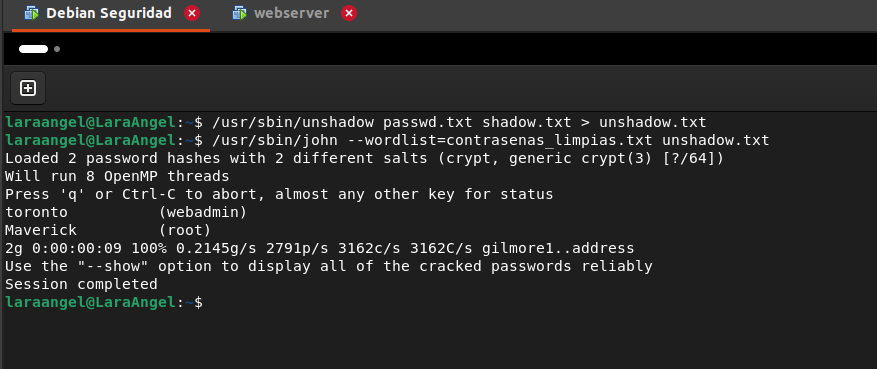
\includegraphics[width=\textwidth]{img/image10.png}
    \caption{Fusion con unshadow y ejecucion de John con el diccionario contrasenas\_limpias.txt.}
    \label{fig:cracking}
\end{figure}

\Needspace{9\baselineskip}
La salida que nos interesa es la siguiente:

\begin{lstlisting}[style=output]
Loaded 2 password hashes with 2 different salts (crypt, generic crypt(3) [?/64])
Will run 8 OpenMP threads
toronto         (webadmin)
Maverick        (root)
Session completed
\end{lstlisting}

Donde en este caso, \texttt{Loaded 2 password hashes} nos dice
que cargo los dos hashes que estamos auditando, y \texttt{2
different salts} indica que cada uno tiene una sal distinta. De
igual forma, la linea de OpenMP muestra que la ejecucion utiliza
ocho hilos de procesamiento.

Despues de esto, la consola nos arroja las contraseñas junto con
el usuario correspondiente, donde para webadmin la contraseña es
\texttt{toronto} y para root es \texttt{Maverick}. En este caso,
el comando se tardo aproximadamente 9 segundos y al terminar nos
arroja \texttt{Session completed}, lo que nos dice que termino
la ejecucion.

Con esto, se vuelve a encontrar la contraseña de webadmin que ya
se conocia desde la practica 3, pero ahora mediante una prueba
local. Ademas de que, tambien se obtiene la contraseña de root,
que no se habia utilizado para conseguir la terminal
administrativa mediante el exploit.

\subsection{Consulta de resultados y comprobacion de la contraseña de root}

Por ultimo, para revisar el resultado de forma ordenada,
ejecutamos el comando con la opcion \texttt{--show}:

\begin{lstlisting}[style=consolaSeguridad]
/usr/sbin/john --show unshadow.txt
\end{lstlisting}

Lo que hace esta opcion es mostrar las contraseñas que John ya
recupero para las cuentas del archivo, en lugar de iniciar otra
vez la busqueda. La salida de nuestra terminal es la siguiente:

\begin{lstlisting}[style=output]
root:Maverick:0:0:root:/root:/bin/bash
webadmin:toronto:1000:1000:webadmin,,,:/home/webadmin:/bin/bash

2 password hashes cracked, 0 left
\end{lstlisting}

\begin{figure}[H]
    \centering
    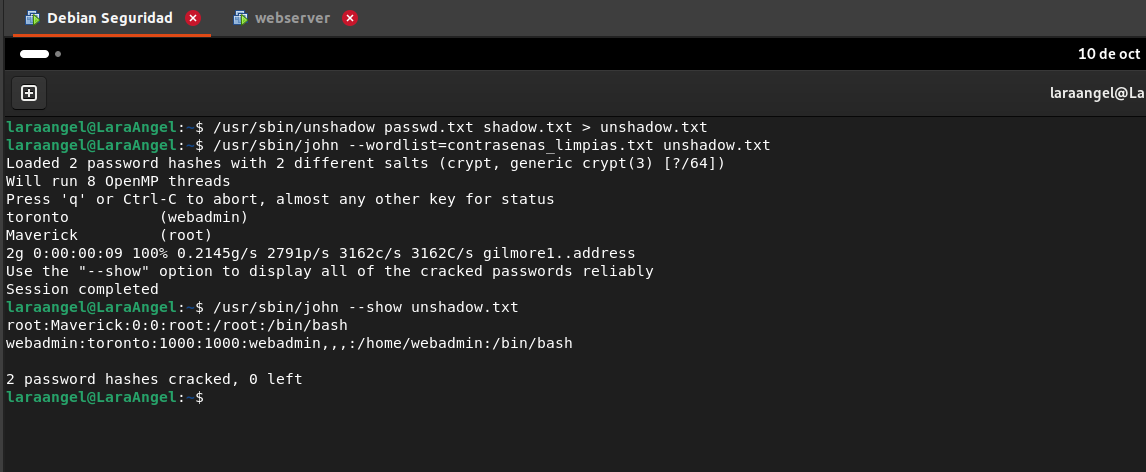
\includegraphics[width=\textwidth,trim=0bp 60bp 0bp 295bp,clip]{img/image11.png}
    \caption{Consulta de las contraseñas recuperadas con john --show.}
    \label{fig:show}
\end{figure}

Donde en este caso, \texttt{2 password hashes cracked, 0 left}
significa que se recuperaron los dos hashes de contraseña
cargados y que no quedaron hashes pendientes en esa entrada.
Esto se refiere a las dos cuentas auditadas, no a que todas las
cuentas de servicios del sistema tengan una contraseña
recuperada.

Ademas de que, para comprobar la contraseña de root, en la
sesion de webadmin del servidor se utiliza lo siguiente:

\begin{lstlisting}[style=consolaSeguridad]
su root
\end{lstlisting}

Despues en la consola se pone la contraseña, siendo
\texttt{Maverick}. Con esto se logra cambiar de webadmin al
usuario root, por lo que se comprueba que la contraseña que nos
dio John es correcta.

\begin{figure}[H]
    \centering
    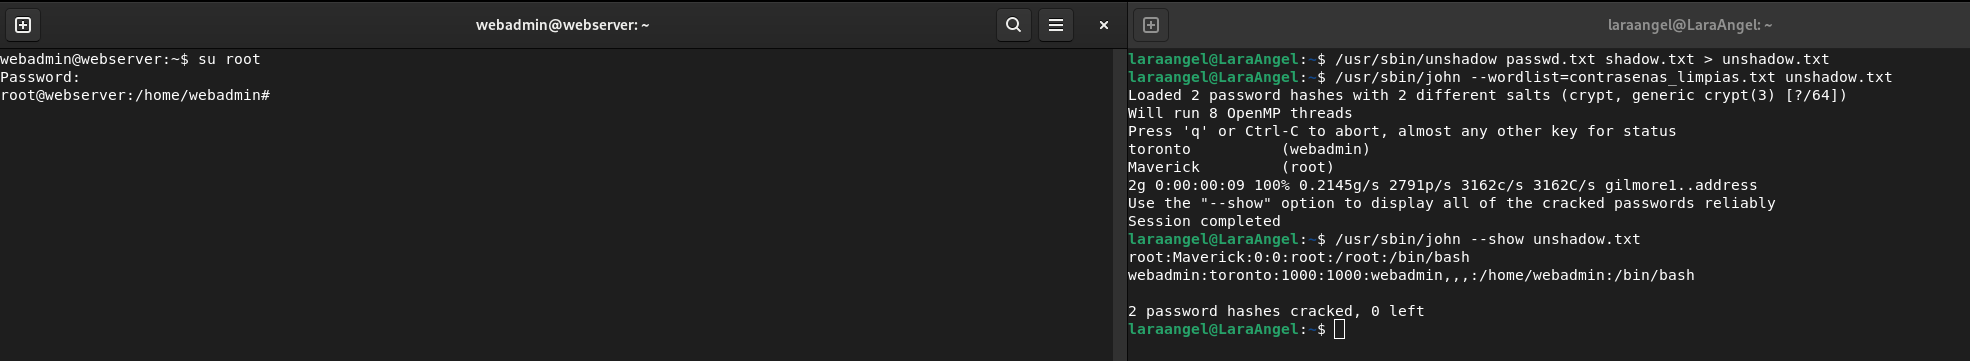
\includegraphics[width=\textwidth,trim=0bp 180bp 855bp 0bp,clip]{img/image12.png}
    \caption{Cambio al usuario root mediante su despues de recuperar su contraseña.}
    \label{fig:su}
\end{figure}

Ahora bien, para este punto ya se ingreso como root utilizando
la contraseña que se obtuvo, esto por que antes se habia
conseguido el acceso por medio de PwnKit y no por medio de la
contraseña.

\section{Actividades}

\subsection{Actividad 1: Hash SHA256 del archivo passwd original}

\textbf{¿Cual es el hash SHA256 del archivo passwd original en
el equipo webserver?}

Para responder esta primera actividad, utilizamos la terminal
root de webserver y calculamos el hash del archivo original.
Para esto, el comando es el siguiente:

\begin{lstlisting}[style=consolaSeguridad]
sha256sum /etc/passwd
\end{lstlisting}

Donde en este caso, el hash que nos devuelve la terminal es:

\begin{lstlisting}[style=hashCredencial]
97b7820d23c5b679f76f2d5a680cf6256dd11739485484ad281527a42adf9ded
\end{lstlisting}

Donde en este caso, el resultado es el mismo que nos dio el
archivo \texttt{passwd.txt} en EvilBox, por lo que se comprueba
que el archivo se copio correctamente.

\subsection{Actividad 2: Hash SHA256 del archivo shadow original}

\textbf{¿Cual es el hash SHA256 del archivo shadow original en
el equipo webserver?}

Ahora bien, para el segundo archivo se realiza el mismo
procedimiento, pero apuntando al archivo shadow del servidor.
Como ya tenemos la terminal con privilegios de root, podemos
leerlo para calcular su resumen:

\begin{lstlisting}[style=consolaSeguridad]
sha256sum /etc/shadow
\end{lstlisting}

El resultado que aparece en la consola es el siguiente:

\begin{lstlisting}[style=hashCredencial]
aa01a017835a9f823ccb1982cd414005bfb0f67f51e3e85dc3716a328eaf4c3e
\end{lstlisting}

De igual forma, este resultado coincide con el que nos dio el
archivo \texttt{shadow.txt} en EvilBox. Cabe recalcar que este
hash corresponde a todo el archivo, y no a la contraseña de un
solo usuario.

\subsection{Actividad 3: Hash de la contraseña del usuario root}

\textbf{¿Cual es el hash de la contraseña del usuario root?}

Para esto, se utiliza el contenido que nos dio el comando
\texttt{cat /etc/shadow}, donde se busca la linea que empieza
con \texttt{root:}. El hash de la contraseña es el segundo
campo, por lo que se toma todo lo que esta entre los primeros
dos separadores de dos puntos.

Donde en este caso, el hash de la contraseña es el siguiente:

\begin{lstlisting}[style=hashCredencial]
$6$x5aaIc6z$ULUN3OLorf.xRY7CRYNbwK7sgg6OSXBy/7psHiVhAKeWfX8Gm2UfUWWXRVGfTCmBRZJeHATpJ03/WSv40DFZJ0
\end{lstlisting}

Ahora bien, se conserva la cadena completa porque \texttt{\$6\$}
identifica SHA512-crypt, \texttt{x5aaIc6z} es la sal y la parte
posterior es el resultado del calculo. Los valores que siguen
despues en la linea de shadow, como \texttt{19685:0:99999:7:::},
son datos de vigencia y no forman parte del hash de contraseña.

\subsection{Actividad 4: Hash de la contraseña del usuario webadmin}

\textbf{¿Cual es el hash de la contraseña del usuario webadmin?}

De igual forma, se utiliza el contenido del archivo shadow, pero
ahora se busca la linea que empieza con \texttt{webadmin:}.
Donde en este caso, el hash tambien empieza con \texttt{\$6\$},
por lo que la contraseña esta guardada con SHA512-crypt.

El segundo campo de esa linea es el siguiente:

\begin{lstlisting}[style=hashCredencial]
$6$1SBe2DKx$Wl.hJsSEuL1iQ0bZksh2Jk89phUWF/hXyYCFaJqL5DB1LR05k.Faje47wy9rk7iUNy9w3sMBTTkmPciPN6L7K/
\end{lstlisting}

Donde en este caso, la sal es \texttt{1SBe2DKx}, que es
diferente de la utilizada para root. Se mantienen las
mayusculas, minusculas y todos los simbolos de la cadena, porque
forman parte del valor que utiliza John para comprobar los
candidatos de contraseña.

\subsection{Actividad 5: Contraseña en claro del usuario root}

\textbf{¿Cual es la contraseña en claro del usuario root?}

Para obtener esta respuesta, se utiliza el resultado de la
ejecucion de John con el diccionario
\texttt{contrasenas\_limpias.txt} y se consulta con el siguiente
comando:

\begin{lstlisting}[style=consolaSeguridad]
/usr/sbin/john --show unshadow.txt
\end{lstlisting}

La salida que nos arroja para el usuario root es la siguiente:

\begin{lstlisting}[style=output]
root:Maverick:0:0:root:/root:/bin/bash
\end{lstlisting}

Por lo que, la contraseña en claro del usuario root es
\textbf{\texttt{Maverick}}, donde la M es mayuscula. Ademas de
que, esta contraseña se comprobo por medio del comando
\texttt{su root}, con el cual se logro ingresar como root en
webserver.

\subsection{Actividad 6: Contraseña en claro del usuario webadmin}

\textbf{¿Cual es la contraseña en claro del usuario webadmin?}

Por ultimo, del mismo resultado de \texttt{john --show} tomamos
la linea correspondiente a webadmin:

\begin{lstlisting}[style=output]
webadmin:toronto:1000:1000:webadmin,,,:/home/webadmin:/bin/bash
\end{lstlisting}

Donde en este caso, la contraseña en claro de webadmin es
\textbf{\texttt{toronto}}, escrita en minusculas. Esta es la
misma que se habia obtenido con Hydra en la practica 3 y con la
que se ingreso por ssh al inicio, por lo que con John se vuelve
a comprobar que es la contraseña correcta.

\newpage
\nocite{*}
\printbibliography[heading=bibintoc, title={Referencias}]
\end{document}
